\section{Building Blocks in \NAME}
In this section, we focus on the query processing in \NAME. 
We start with a general homomorphic SQL paradigm and 
propose our novel algorithms: 
homomorphic comparison and homomorphic repack, 
which are vital building blocks of homomorphic query evaluation. 
The two algorithms are also of 
independent interest in the FHE research community.
Moreover, we provide the translation mechanism of 
other complex SQL operators into FHE circuits.

\subsection{Overview}
\NAME works on the encrypted table $\mathcal{CT}$, that is, 
a set of RLWE ciphertexts 
$(ct_1, ct_2, ..., ct_{\lvert \mathcal{T} \rvert_{c}})$.
On a high level, the evaluation of encrypted query 
$\mathcal{CQ} = (cp_{1}, cp_{2}, ... ,cp_{\lvert \mathcal{Q} \rvert}, B, G)$ 
on $\mathcal{CT}$  
can be summarized in the following steps.
In \cref{algo: query_evaluation}, we detail the extract algorithm
for homomorphic query evaluation and illustrate a plaintext process
in \cref{fig: query_eva}.

\textbf{1) Line 1-11, homomorphic filtering}: 
For each encrypted predicate $cp_i$, 
$i \in (1, 2, ..., \abs{\mathcal{Q}})$, 
we first get the attribute index of the predicate $d$ 
and the comparison operator $op$
($\geq, \leq, ==, >, <$) of the predicate.
Here, the $ct_d$ represents the RLWE ciphertext which
encrypts the matching column in $\mathcal{T}$
and the $cp_i$ refers to the RLWE ciphertext of the predicate value.
Then, we sample extract the RLWE ciphertexts $ct_d$ and $cp_i$, 
and get two LWE ciphertext vectors
$\mathbf{ct_d}$ and $\mathbf{cp_i}$ wich size $\abs{\mathcal{T}}_{r}$.
For each LWE ciphertext $ct_d[j]$and $cp_i[j]$, 
we perform \texttt{HomCom} of the two LWE ciphertext
with the comparison operator $op$
and get the encrypted comparison result $comp_{i,j}$.
Next, we evaluate the logic gate between different predicates 
using \texttt{HomGate}.
After the $\abs{\mathcal{Q}}$ loops, 
we calculate the filtering results 
$(fl_{\abs{\mathcal{Q}}, 1},
fl_{\abs{\mathcal{Q}}, 2}...,
fl_{\abs{\mathcal{Q}}, \abs{\mathcal{T}}_{r}})$
where each $fl_{\abs{\mathcal{Q}}, i}$ is an LWE
ciphertext which encrypts $1$ or $0$, 
indicating the $i$-th row of $\mathcal{T}$
is selected or not.

\textbf{2) Line 12, ciphertext conversion}:
After the homomorphic filtering, we get $\abs{\mathcal{T}}_{r}$
LWE ciphertexts which encrypt the filtering results.
The $\texttt{LWEsPack}$
packs $\abs{\mathcal{T}}_{r}$ into a RLWE ciphertext $fl$
for latter homomorphic aggregation.

\textbf{3) Line 13-23, homomorphic aggregation}:
The aggregation process computes the group function 
on the filtered rows.
For each aggregation filed $g_i$, 
we get the attribute index $d = g(a)_i$
and the aggregation function $f_i = g(f)_i$.
As the filtering result $fl$ is in coefficient format, 
we directly perform the aggregate function when $f_i$ supports 
coefficient format computation.
Otherwise, we first evaluate the \texttt{CoeffToSlot} 
to convert $fl$ to $\hat{fl}$ slot format ciphertext $\hat{fl}$
and then computes the $f_i$ in slot format.

\begin{figure}[htbp]
   \begin{center}
   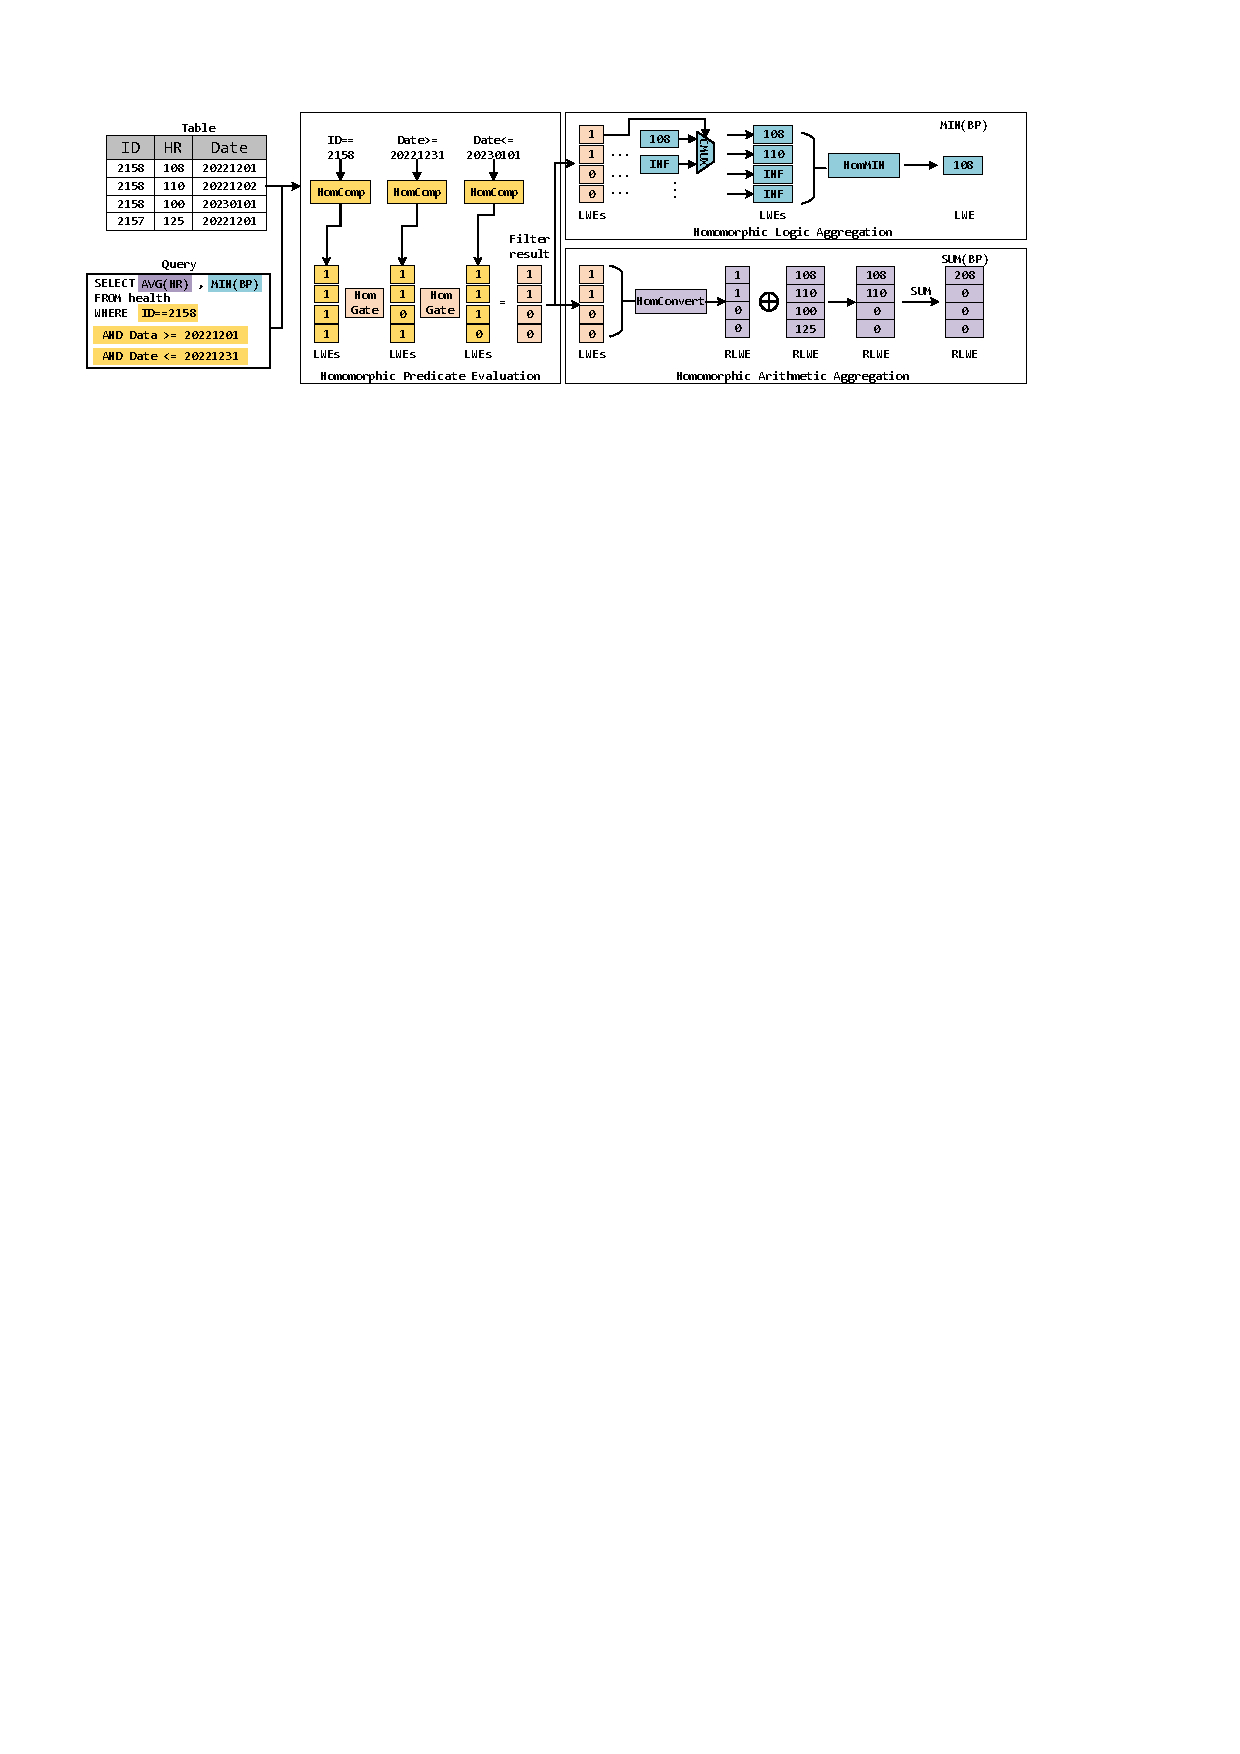
\includegraphics[width=0.9\linewidth]{figure/query.pdf}
   \end{center}
    \vspace{-0.5em}
      \caption{A plaintext illustration in query evaluation.} 
   \label{fig: query_eva}
   \vspace{-0.5em}
\end{figure}

\begin{algorithm}[htbp]
    % \tiny
    \caption{Homomorphic Query Evaluation \texttt{HomQuery}}
    \label{algo: query_evaluation}
    \SetKwInOut{Input}{Input}\SetKwInOut{Output}{Output}\SetKwInOut{Return}{Return}
    \Input{Ecrypted table $\mathcal{CT}=
    (ct_{1}, ct_{2}, ... , ct_{\lvert \mathcal{T} \rvert_{c}})$, 
    Encrypted Query $\mathcal{CQ}=
    (cp_{1}, cp_{2}, ... ,cp_{\lvert \mathcal{Q} \rvert}, B, G)$}
    \Output{A set of (R)LWE cipher $\mathcal{CR}
     = (cr_1, cr_2, ..., cr_{\lvert G \rvert})$.}
     Set $fl_{0,j} = {\rm LWE}(1)$ 
     for $j \in (1,2,...,\lvert \mathcal{T} \rvert_{r})$ and $b_0 = AND$\\
    \For{$i = 1$ \KwTo $\lvert \mathcal{Q} \rvert$}
    {
        $d = cp(a)_i$ \tcp*{Attribute index of $cp_i$} \\
        $op = cp(o)_i$ \tcp*{Operator of $cp_i$} \\
        $\mathbf{ct_d} = \texttt{SampleExtract}(ct_{d})$ 
        \tcp*{$\lvert \mathcal{T} \rvert_{r}$ LWEs}\\
        $\mathbf{cp_i} = \texttt{SampleExtract}(cp_{i})$ \\
        \For{$j = 1$ \KwTo $\lvert \mathcal{T} \rvert_{r}$}
        {
            $comp_{i,j} = \texttt{HomCom}
            (\mathbf{ct_d}[j], \mathbf{cp_i}[j],op)$ \\
            $fl_{i,j} = \texttt{HomGate}(fl_{i-1, j}, comp_{i,j}, b_{i-1})$ \\
        }
    }
    $fl = \texttt{LWEsPack}(fl_{\abs{Q}, 1},fl_{\abs{Q}, 2}...,fl_{\abs{Q}, \abs{T}})$ \tcp*{A RLWE} \\
    \For{$i = 1$ \KwTo $\lvert G \rvert$}
    {
        $d = g(a)_i$ \\
        $f_i = g(f)_i$ \\
        \eIf{$g_i$ is support coeffcient}
        {
            $cr_i = \texttt{Homfun}(fl, ct_d, f_i, \texttt{Coeff})$ \\
        }
        {
            $\hat{ct_d} = \texttt{SlotToCoeff}(ct_d)$ \\
            $\hat{fl} = \texttt{SlotToCoeff}(fl)$ \\
            $cr_i = \texttt{Homfun}(\hat{fl}, \hat{ct_d}, f_i, \texttt{Slot})$ \\
        }
    }
    \Return{$\mathcal{CR}
     = (cr_1, cr_2, ..., cr_{\abs{G}})$}
\end{algorithm}

\subsection{Efficient Homomorphic Comparison}
In this section, we propose our novel homomorphic comparison algorithm
\texttt{HomCom} where both the inputs are ciphertexts.
As shown in \cref{algo: query_evaluation}, \texttt{HomCom}
is the essential part of homomorphic filtering.

\subsubsection{Difficulties in improving the performance of homomorphic comparison}
Most of the existing works~\cite{heda, pegasus,largeprecision} start with 
the simple fact that the comparison of two encrypted numbers $a$ and $b$
can be evaluated by extracting the most significant bit (MSB) from $a-b$.
For instance, to evaluate $a \geq b$, we compute $a -b$ and homomorphically
extract the MSB of the reduction result. 
The result only encrypts a value of $0$ when $a \geq b$ and 
a value of $1$ when $a \textless b$. 
However, the homomorphic MSB extraction based on PBS 
is limited to small precision (less than 6 bits). 
The main obstacle is that the precision of PSB is strictly 
related to the parameters of the test vector 
as we mentioned in ...
In order to obtain high precision, one adopts a test vector with a large
degree or represents a high-bit ciphertext with several low-bit ciphertexts, 
which results in an increased computation cost or storage consumption.


\subsubsection{Our solution via discarding invalid bit}
In this work, we propose our innovative homomorphic comparison method
which enables us to convert a high-precision comparison to 
a low-precision comparison by iterating PLB. 
Our critical insight is that, in principle, the output of 
homomorphic MSB extraction depends only on the first bit 
of the plaintext, so we can homomorphically \textit{discard}
the invalid bits and consider the result as low-precision 
ciphertext with a larger scale. In \cref{algo: 2kHMSB}, we detail the exact 
algorithm for constructing a $2k$-bit MSB extraction using
$(k+1)$-bit MSB extractions and PBS.

We start with a standard homomorphic MSB extraction algorithm 
${\rm HMSB}_{k}$ in Pegasus~\cite{pegasus} and HEDA~\cite{heda} 
that homomorphically extract the MSB of a $k$-bit ciphertext. 
In \cref{algo: kHMSB}, it can be seen that the standard 
MSB extraction algorithm basically follows the PBS procedure 
and the precision is limited due to the degree of the test vector.

We construct a ${\rm HMSB}_{2k}$ as follows and sketch the process in 
\cref{fig: comparison}. Given an input ciphertext 
$ct_{I} = {\rm LWE}_{n,q}(m)$, where $m=2^{k}\cdot m_1 + m_0$. We first 
shift the input ciphertext and get $ct_{1}$. After the shifting process, 
the most $(k-1)$bits of $m_{1}$ have been 
moved as shown in \cref{fig: comparison}. 
However, to correctly
bootstrap a ciphertext, the MSB of the encrypted plaintext needs to be set to zero.
To address this problem, we should remove the MSB of plaintext.
By applying ${\rm HMSB}_{k+1}$ to $ct_{1}$, we get 
$ct_{2} = {\rm LWE}_{n,q}(2^{2k-1}{\rm LSB}(m_{1}))$, which
encrypts the LSB of $m_{1}$. 

Then, we substract $ct_{2}$ from $ct_{1}$ and get $ct_{3}$ where 
$ct_{3}$ which encrypts $2^{k-1}m_{0}$. After steps 2 and 3, we 
have discarded the MSB of the encrypted plaintext and we can apply 
PBS to $ct_{3}$. By applying PBS to $ct_{3}$, we get $ct_{4} = {\rm LWE}_{n,q}(m_0)$. And then, computing $ct_{I} - ct_{4}$, we get 
$ct_{5} = {\rm LWE}_{n,q}(2^{k}m_1)$. Until now we have removed the 
least $k$ bits of $m$. Finally, by applying ${\rm HMSB}_{k}$ 
to $ct_{5}$, we obtain $ct_{O} = {\rm LWE}_{n,q}({\rm MSB}(m))$.

\begin{algorithm}[t!]
    % \tiny
    \caption{The standard $k$-bit homomorphic MSB Extraction}
    \label{algo: kHMSB}
    \SetKwInOut{Input}{Input}\SetKwInOut{Output}{Output}\SetKwInOut{Return}{Return}
    \Input{A LWE ciphertext $ct_{I} = {\rm LWE}^{n,q}_{\mathbf{s}}(m) 
    = (b, \mathbf{a})$, where $m \ in [0, 2^{k} -1]$.}
    \Input{A constant $\mu = q / 4$.}
    \Input{A bootstrapping key $\mathbf{BK}$, where 
    $\mathbf{BK}\left[i\right] = RGSW^{N,q}_{s}(s[i])$, for $i \in [1,n]$}
    \Output{A LWE ciphertext $ct_{O} = {\rm LWE}_{n,q}({\rm MSB}(m))$.}
    $b \leftarrow \lfloor \frac{2N}{q}b \rceil$ 
    and $\mathbf{a} \leftarrow \lfloor \frac{2N}{q}\mathbf{a} \rceil$ \\
    $\mathbf{v} \leftarrow \mu \cdot (1 + x^2 + x^3 + ... + x^{N-1}) $ \\
    $ACC \leftarrow {\rm BlindRotate}(v, b, \mathbf{a}, \mathbf{BK})$ \\
    $ct_{O} = (b', \mathbf{a'}) = {\rm SampleExtract}^{0}(ACC)$ \\
    \Return{$ct_{O} = (b' + \mu, \mathbf{a}) 
    = {\rm LWE}_{n,q}({\rm MSB}(m))$}
\end{algorithm}

\begin{algorithm}[t!]
    % \tiny
    \caption{Constructing $2k$-bit MSB Extraction 
            using $(k+1)$-bit MSB Extraction}
    \label{algo: 2kHMSB}
    \SetKwInOut{Input}{Input}\SetKwInOut{Output}{Output}\SetKwInOut{Return}{Return}
    \Input{A LWE ciphertext $ct_{I} = {\rm LWE}_{n,q}(m)$, where $m=2^{k}\cdot m_1 + m_0$.}
    \Output{A LWE ciphertext $ct_{O} = {\rm LWE}_{n,q}({\rm MSB}(m))$.}
    $ct_{1} \leftarrow 2^{k-1}ct_{I}$ \tcp*{$ct_{1} = {\rm LWE}_{n,q}(2^{2k-1}{\rm LSB}(m_1) + 2^{k-1}m_0)$} \\
    $ct_{2} \leftarrow {\rm HMSB}_{k+1}(ct_{1}) $ 
    \tcp*{$ct_{2} = {\rm LWE}_{n,q}(2^{2k-1}{\rm LSB}(m_{1}))$} \\
    $ct_{3} \leftarrow ct_{1} - ct_{2}$ 
    \tcp*{$ct_{3} = {\rm LWE}_{n,q}(2^{k-1}m_0)$} \\
    $ct_{4} \leftarrow {\rm PBS}(ct_{3})$ 
    \tcp*{$ct_{4} = {\rm LWE}_{n,q}(m_0)$} \\
    $ct_{5} \leftarrow ct_{I} - ct_{4}$ 
    \tcp*{$ct_{5} = {\rm LWE}_{n,q}(2^{k}m_1)$} \\
    $ct_{O} \leftarrow {\rm HMSB}_{k}(ct_{5})$
    \tcp*{$ct_{O} = {\rm LWE}_{n,q}({\rm MSB}(m))$} \\
    \Return{$ct_{O} = {\rm LWE}_{n,q}({\rm MSB}(m))$}
\end{algorithm}

\begin{figure*}[t!]
   \begin{center}
   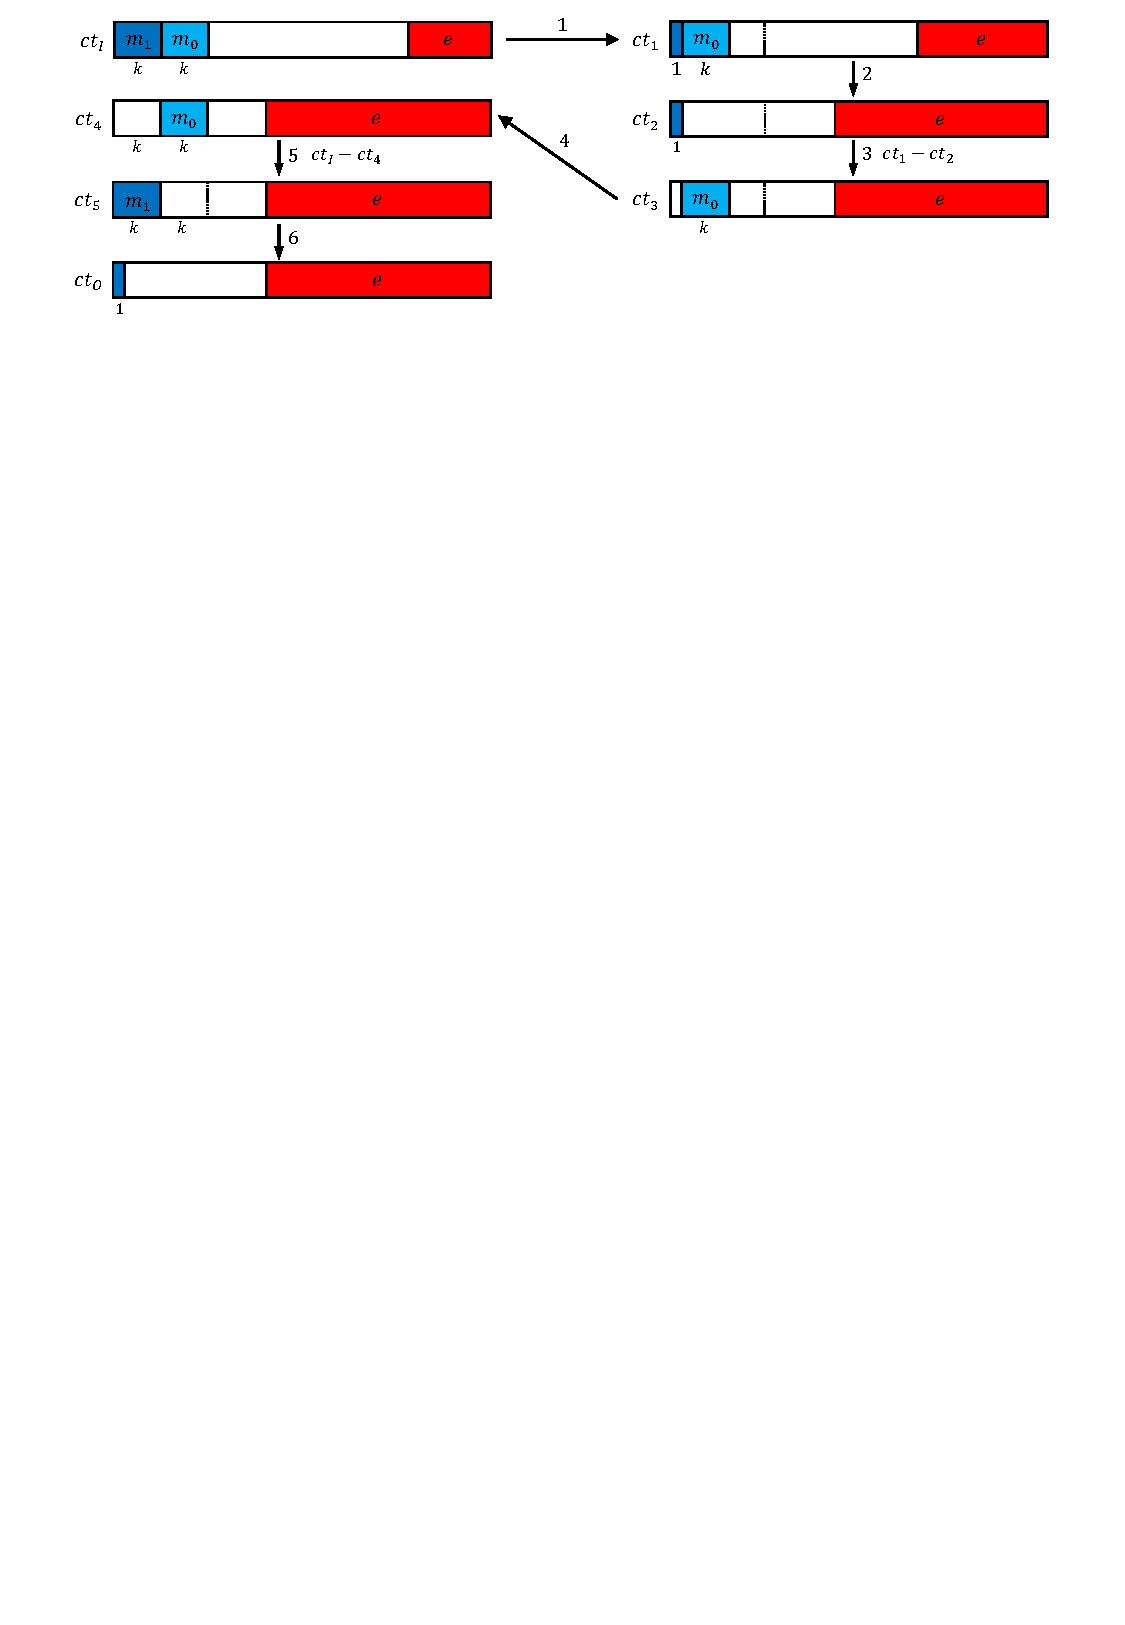
\includegraphics[width=0.9\linewidth]{figure/comparison.pdf}
   \end{center}
    \vspace{-0.5em}
      \caption{A plaintext illustration in \cref{algo: 2kHMSB}. 
      Each rectangle represents a decrypted plaintext while the left is 
      the most significant bit.
      The blue-colored region is the bits occupied by the message, 
      the red-colored field is the bits filled with noise, 
      and the white part is the bits set to zero.} 
   \label{fig: comparison}
   \vspace{-0.5em}
\end{figure*}

\subsubsection{Generality algorithm}
Furthermore, we propose an algorithm for 
constructing a $(t+1)\cdot k$-bit MSB extraction 
by $tk$-bit and $(k+1)$-bit MSB extractions and PBS.
Given an input ciphertext $ct_{I} = {\rm LWE}_{n,q}(m)$, 
where $m=\sum_{i = 0}^{t}2^{ik} \cdot m_{i}$.
As shown in \cref{algo: tkHMSB}, in generality, we shift the ciphertext
$(tk-1)$bits to move the most $(tk-1)$bits of $m$ 
and reserve the least $(k+1)$bits. 
The goal of the next four steps (line 2-5) is to move $m_{0}$ from $m$ 
in an encrypted form, which is the same as \cref{algo: 2kHMSB}. 
After that, we get the ciphertext $ct_{5}={\rm LWE}_{n,q}(m-m_0)$ and the 
$m-m_{0}$ can be regarded as a $tk$-bit precision plaintext.
By adopting ${\rm HMSB}_{tk}$ to $ct_{5}$, we obtain $ct_{O}$
that encrypts the MSB of $m$.



\begin{algorithm}[t!]
    % \tiny
    \caption{Constructing ${\rm HMSB}_{(t+1)k}$ using ${\rm HMSB}_{tk}$ and
    ${\rm HMSB}_{k+1}$}
    \label{algo: tkHMSB}
    \SetKwInOut{Input}{Input}\SetKwInOut{Output}{Output}\SetKwInOut{Return}{Return}
    \Input{A LWE ciphertext $ct_{I} = {\rm LWE}_{n,q}(m)$, where 
    $m=\sum_{i = 0}^{t}2^{ik} \cdot m_{i}$.}
    \Output{A LWE ciphertext $ct_{O} = {\rm LWE}_{n,q}({\rm MSB}(m))$.}
    $ct_{1} \leftarrow 2^{tk-1}ct_{I}$ 
    \tcp*{$ct_{1} = {\rm LWE}_{n,q}(2^{(t+1)k-1}{\rm LSB}(m_1) + 2^{tk-1}m_0)$} \\
    $ct_{2} \leftarrow {\rm HMSB}_{k+1}(ct_{1}) $ 
    \tcp*{$ct_{2} = {\rm LWE}_{n,q}(2^{(t+1)k-1}{\rm LSB}(m_{1}))$} \\
    $ct_{3} \leftarrow ct_{1} - ct_{2}$ 
    \tcp*{$ct_{3} = {\rm LWE}_{n,q}(2^{tk-1}m_0)$} \\
    $ct_{4} \leftarrow {\rm PBS}(ct_{3})$  
    \tcp*{$ct_{4} = {\rm LWE}_{n,q}(m_0)$} \\
    $ct_{5} \leftarrow ct_{I} - ct_{4}$  
    \tcp*{$ct_{5} = {\rm LWE}_{n,q}(m-m_{0})$} \\
    $ct_{O} \leftarrow {\rm HMSB}_{tk}(ct_{5})$ 
    \tcp*{$ct_{O} = {\rm LWE}_{n,q}({\rm MSB}(m))$} \\
    \Return{$ct_{O} = {\rm LWE}_{n,q}({\rm MSB}(m))$}
\end{algorithm}


\subsubsection{Homomorphic Comparison in EDBMS}
Let $ct_1$ and $ct_2$ be the two LWE ciphertexts
that encrypt $pt_1$ and $pt_2$.
\texttt{HomCom}$(ct_1, ct_2, \texttt{op})$ 
outputs an LWE ciphertext encrypting $1$
if the predicate $pt_1$ \texttt{op} $p_2$ is True 
and $0$ if $pt_1$ \texttt{op} $p_2$ is False.
The \texttt{HomCom} algorithm
can be easily constructed by \texttt{HMSB}
and homomorphic gates.
We list detailed the specific procedure in \cref{tab:homcom}.

\begin{table}[htbp] 
    \centering
    \caption{Constructing \texttt{HomCom} using \texttt{HMSB}}
    \vspace{-0.5em}
        \begin{tabular}{cc}
            \toprule
            \texttt{HomCom} & Operation \\
            \midrule
            $\texttt{HomCom}(c_1, c_2, \geq)$ & 
            $\texttt{NOT}(\texttt{HMSB}(c1-c2))$\\
            $\texttt{HomCom}(c_1, c_2, >)$ & 
            $\texttt{HMSB}(c2-c1)$ \\
            $\texttt{HomCom}(c_1, c_2, \leq)$ & 
            $\texttt{NOT}(\texttt{HMSB}(c2-c1))$\\
            $\texttt{HomCom}(c_1, c_2, <)$ & 
            $\texttt{HMSB}(c1-c2)$ \\
            $\texttt{HomCom}(c_1, c_2, ==)$ & 
            $\texttt{HomCom}(c_1, c_2, \geq)$  
            \texttt{AND} $\texttt{HomCom}(c_1, c_2, \leq)$ \\
            
            
            \bottomrule
        \end{tabular}
    \label{tab:homcom}
\end{table}

\subsubsection{Compare to other solutions}
We compare our algorithm with other related solutions in theory
and propose more experimental analysis in \cref{eva: microbenchmarks}.
We emphasize that all of the methods discussed below 
have their own advantages and 
method selection depends on the application.
General approaches like Pegasus~\cite{pegasus} and the method 
of Liu~\cite{largeprecision} focus on arbitrary homomorphic logic
functions by proposing efficient or large-precision PBS algorithms
while \NAME only concentrates on the homomorphic comparison.
SortingHat~\cite{sortinghat} proposes an efficient plaintext-ciphertext 
comparison algorithm but shows poor performance on ciphertext-ciphertext
comparison. The method of Antonio~\cite{revisiting} encrypts the input 
in a bit-wise format to construct fast and high-precision
homomorphic comparison. After the bit-by-bit comparisons, it 
gets an LWE ciphertext encrypting $\{-1,0,1\}$, 
respectively representing the \texttt{<}, \texttt{==} and \texttt{>}.
However, Antonio's approach~\cite{revisiting} does not support 
the encrypted database scenarios as the result of the comparison 
could not perform logic gate operation between various predicates.

Another technical route is based on the polynomial approximations 
using the RLWE ciphertexts(BFV, BGV, and CKKS)~\cite{ckkscomparison, aphadb}.
These methods can quickly evaluate lots of ciphertext comparisons 
by the advantage of the SIMD packing.
Nonetheless, both of their methods fail to achieve elastic encrypted 
database as the method of Cheon~\cite{ckkscomparison} could not 
support homomorphic comparison \texttt{==} and the method of 
Kortekass~\cite{aphadb} support bounded filtering predicates 
due to the noise growth of RLWE ciphertext 
as we discussed in \cref{pre:he_type}.
To be more specific, in ~\cite{aphadb}, the user has to encrypt the 
data in a predefined depth and could not process 
encrypted queries that are more complicated than such depth.
We list the qualitative comparisons between existing methods and 
provide quantitative comparisons in \cref{eva: microbenchmarks}.

\begin{table*}[htbp] 
    \centering
    \caption{Qualitative comparisons between existing homomorphic comparison algorithms in the case of an encrypted database.}
    \vspace{-0.5em}
        \begin{tabular}{cccccccc}
            \toprule
            & Kortekaas~\cite{aphadb}
            & Antonio~\cite{revisiting}
            & Pegasus~\cite{pegasus} 
            & Liu~\cite{largeprecision}
            & SortingHat~\cite{sortinghat} 
            & Cheon~\cite{ckkscomparison} 
            & Ours\\
            \midrule
            Complete operators & \yeah & \nope & \yeah & \yeah & \yeah & \nope& \eyeah \\
            16bit-precision & \yeah & \yeah & \nope & \yeah & \yeah & \yeah & \eyeah \\
            32bit-precision & \yeah & \yeah & \nope & \nope & \yeah & \nope & \eyeah \\
            Predicate evaluation & \yeah & \nope & \yeah & \yeah & \yeah & \yeah & \eyeah \\
            Unbounded predicates & \nope & \nope & \yeah & \yeah & \yeah & \nope & \eyeah\\
            Efficiency & High & High & Low & Low & Low & High & High\\
            Storage & High & High & Low & Low & High & High & Low\\
            \bottomrule
        \end{tabular}
    \label{tab:homcom}
\end{table*}

\subsection{High-precision Ciphertext Conversion}
After the homomorphic filtering, the $\abs{\mathcal{T}}$ LWE ciphertexts 
have to be packed in an RLWE ciphertext for later homomorphic aggregation.
In this section, we propose our novel homomorphic ciphertext conversion
algorithm \texttt{LWEsPack} for encrypted database.

\subsubsection{Limitations in existing methods}
Existing representative works in ciphertext conversion 
include Pegasus~\cite{pegasus} and 
the method of Chen~\cite{conversionhaochen}.
The key idea of Pegasus~\cite{pegasus} in ciphertext conversion 
consists of homomorphically evaluating LWE partial decryption as well as 
homomorphically evaluating modulo $q$ on an RLWE ciphertext encrypting secret key.
Both two operations can be achieved 
by arithmetic homomorphic circuits~\cite{helib,ckksbootsparse,ckksbootvariance}.
Taking advantage of SIMD packing arithmetic homomorphic circuits, 
Pegasus~\cite{pegasus}
performs fast ciphertext conversion but low-precision 
due to the noise growth in homomorphic arithmetic circuits.
The method of Chen~\cite{conversionhaochen} evaluates
homomorphic automorphisms~\cite{helib} recursively
to pack the LWE ciphertexts into the coefficient of an RLWE ciphertext.
This approach achieves high-precision packing but is 
limited to a small size.
When the packing size of LWE ciphertexts is large, 
the latency of ~\cite{conversionhaochen} is still very high.
However, in an encrypted database, we want to achieve an efficient 
and high-precision \texttt{LWEsPack} algorithm.

\subsubsection{Our solution via precision revision}
In \NAME, we propose our creative homomorphic ciphertext conversion method
for homomorphically encrypted database
which achieves low latency and high precision.
Our critical insight is that, in a homomorphically encrypted database, 
the filtering results are in a certain range ($0$ or $1$), 
thus we can correct the error on low-precision ciphertext to 
obtain high-precision ciphertext.
To be more specific, 
we evaluate the \texttt{Round} function homomorphically on
the low-precision packed RLWE ciphertext
$ct = \reg{RLWE}(\mathbf{m})$ ($\mathbf{m}[i] = 0\pm e$ or $1\pm e$)
to get $ct' = 
\reg{RLWE}(\mathbf{m'})$ ($\mathbf{m'}[i] = \texttt{Round}(\mathbf{m}[i])$
with a lower-norm noise.

\subsubsection{Specific algorithm}
In \cref{algo: lwespack}, we detailed the exact algorithm
for our homomorphic conversion \texttt{LWEsPack}.
The algorithm involves the following steps:

\step{Line 1-3, Linear Transform}:
Given $N$ LWE filtering result ciphertexts $ct_1, ct_2, ...,ct_N$
where $ct_i = \reg{LWE}_{\mathbf{s}}^{n,q}(m_i) = (b_i, \mathbf{a_i})$.
We first rearrange the ciphertexts and construct a ciphertext-matrix
$\mathbf{A} = [\mathbf{a_1}, \mathbf{a_2}, ..., \mathbf{a_N}]^{T} 
\in \mathbb{Z}_{q}^{N \times n}$ and a ciphertext vector 
$\mathbf{b} = [b_1, b_2, ...,b_N] \in \mathbb{Z}_{q}^{N}$.
Then we evaluate the matrix-vector multiplication algorithm
\texttt{HomMVMul} to get $ct = \reg{RLWE}^{N,Q_1}_{\Tilde{s}}(\mathbf{A}\mathbf{s})$.
Followed by a homomorphic addition with the vector $\mathbf{b}$, 
we perform the LWE decryption formula $\mathbf{A}\mathbf{s}+\mathbf{b}$
except for the modulo function.
% While there is a vast amount of prior work~\cite{helib, gazelle, haochenONN, pegasus}
% on HE for matrix-vector multiplication, 
% none take a generally efficient approach in all applications.
% Need to discuss

\step{Line 4, Modulo $q$}:
After the homomorphic linear transform, we obtain ciphertext 
of $\mathbf{A}\mathbf{s}+\mathbf{b} = \mathbf{m} + tq$.
The \texttt{HomMod} evaluates the \texttt{mod} $q$ function homomorphically
on $ct_2$ to obtain $ct = \reg{RLWE}^{N,Q_2}_{\Tilde{s}}(\mathbf{m+e})$.
The homomorphic modular reduction function is a central part
of CKKS bootstrapping~\cite{ckksbootstrap}, 
which is a cryptography puzzle of the FHE research community.
A lot of recent work~\cite{ckksbootsparse, ckksbootvariance, sinemod}
propose their own algorithm to solve it,
and we adapt the approach from ~\cite{ckksbootsparse}
as this is not the research part of this paper.

\step{Line 5, Generate Approximate Round Function}:
As it is not easy to  evaluate a round function
via homomorphic arithmetic circuits directly, 
we generate a high-degree polynomial to 
approximate the target round function.
Specially, given an interval $[u,v]$ and a predefined 
precision parameter $\delta$, we want to obtain
a polynomial $p(x) =  {\textstyle \sum_{i=0}^{n-1}}a_ix^i $ satisfies the \cref{formula: appro}.
\begin{equation}
\forall x \in [u,v],  |p(x)-\left [x  \right ] | < 2^{-\delta } \label{formula: appro}
\end{equation}
This question is a classical problem in approximation theory.
Based on the equioscillation theorm~\cite{equioscillation}, if $p(x)$
is the best possible approximation of the round function
if and only if 
it satisfies:
\begin{equation}
\exists x_0 \leq ... x_i ... \leq x_n \in [u,v], 
p(x_i) - [x_i] = \epsilon(-1)^{i}|p(x) - [x]|_{\infty} 
\label{formula: equioscillation}
\end{equation}
where $\epsilon$ = $\pm 1$.
Taking \cref{formula: equioscillation} as the judgment condition, 
we could construct the Remez iteration algorithm~\cite{remez} to 
obtain the polynomial $p(x)$ meets the requirement of \cref{formula: appro}.

\step{Line 6, Homomorphic Round Evaluation}:
After generating the approximated round function $p(x)$, we need to 
evaluate the $p(x)$ homomorphically.
As $p(x) =  {\textstyle \sum_{i=0}^{n-1}}a_ix^i $ is a type of 
polynomial functions, it could be implemented efficiently 
by homomorphic arithmetic circuits as we introduced in \cref{pre:he_circuits}.
Moreover, expressing the approximated function $p(x)$ 
in a Chebyshev basis~\cite{chebyshevbasis}
could optimize the evaluation process with a less 
number of ciphertext multiplication~\cite{
improvedboot, betterboot, ckksbootsparse, inverseboot, errorboot}.  

\begin{algorithm}[htbp]
    % \tiny
    \caption{Homomorphic conversion \texttt{LWEsPack}}
    \label{algo: lwespack}
    \SetKwInOut{Input}{Input}\SetKwInOut{Output}{Output}\SetKwInOut{Return}{Return}
    \Input{$N$ LWE ciphertexts $(ct_1, ct_2, ...,ct_N)$ where 
    $ct_i = {\rm LWE}^{n,q}_{\mathbf{s}}(m_i) = (b_i, \mathbf{a_i})$
    and $m_i = 0/1$. }
    \Input{A conversion key 
    $\reg{\mathbf{CK}} = \reg{RLWE}^{N,Q}_{\Tilde{s}}(\mathbf{s})$, 
    where $\Tilde{s}_j = \mathbf{s}[j]$ for $j \in \mathbb{Z}_n$.}
    \Input{A precision parameter $\delta$, range parameter $(u,v)$}
    \Output{An RLWE ciphertext $ct = \reg{RLWE}^{N,Q'}_{\Tilde{s}}(\Tilde{m})$,
    where $\Tilde{m}_i = m_i$ for $i \in \mathbb{Z}_{N}$}
     Let $\mathbf{b} = [b_1, b_2, ...,b_N]$, 
     $\mathbf{A} = [\mathbf{a_1}, \mathbf{a_2}, ..., \mathbf{a_N}]^{T} \in \mathbb{Z}_{q}^{N \times n}$\\
     $ct_1 = \texttt{HomMVMul}(\mathbf{A},CK)$.
     \tcp*{$ct_1 = \reg{RLWE}^{N,Q_1}_{\Tilde{s}}(\mathbf{A}\mathbf{s})$} \\
     $ct_2 = \texttt{HomAdd}(ct_1, \mathbf{b})$
     \tcp*{$ct_2 = \reg{RLWE}^{N,Q_1}_{\Tilde{s}}(\mathbf{A}\mathbf{s} + \mathbf{b})$} \\
     $ct_3 = \texttt{HomMod}(ct_2, q)$
     \tcp*{$ct_3 = \reg{RLWE}^{N,Q_2}_{\Tilde{s}}(\mathbf{m+e})$} \\
     $P = \texttt{ApproRound}(u,v,\delta) = (p_1(x), p_2(x), ...,p_d(x))$ \\
     $ct = \texttt{HomPoly}(ct_3, P)$
     \tcp*{$ct = \reg{RLWE}^{N,Q_3}_{\Tilde{s}}(\texttt{sign}(\mathbf{m-\frac{1}{2}}))$} \\
    \Return{$ct = \reg{RLWE}^{N,Q'}_{\Tilde{s}}(\mathbf{m})$}
\end{algorithm}

% \subsubsection{Arithmetic }


\subsection{Homomorphic Logic Aggregation}
Existing homomorphically encrypted database~\cite{aphadb} only supports 
arithmetic aggregation (e.g., \texttt{SUM}) functions.
In this section, we describe how \NAME 
supports logic aggregation function.
We propose our novel 
homomorphic \texttt{MAX/MIN} aggregation algorithm for encrypted database
and construct \texttt{ORDER BY} SQL operator based on it.

\subsubsection{Difficulties in homomorphic \texttt{MAX/MIN} aggregation}
While there exists some prior work~\cite{ckkscomparison, pegasus} 
on HE for \texttt{MAX/MIN} evaluation, 
none could be applied to a homomorphically encrypted database, 
which is essential for addressing two major obstacles.
The first is how to evaluate \texttt{MAX/MIX} only on filtered rows.
In a homomorphically encrypted database, the selected entries as well as 
the number of selected entries are protected during the whole process.
% For instance, we could not distinguish the ciphertext of selected entries 
% between all entry ciphertexts
% $(ct_1, ct_2, ...,ct_{\abs{\mathcal{T}}_r})$.
Thus, it is hard to only perform \texttt{MAX/MIN} on 
the ciphertexts of selected entries.
The second lies in the tussle between latency and precision.
The method of ~\cite{ckkscomparison} suffers from large parameters
which lead to high latency and the method of ~\cite{pegasus}
has limited precision ($< 12$ bit).

\subsubsection{Our solution via elastic selector}
We propose our innovative method to address the two obstacles.
For the first obstacle, we define a gigantic (infinitesimal) ciphertext
and use the encrypted filtering result 
as a control signal of the homomorphic binary selector \texttt{CMUX}
to select between the initial ciphertext and 
the gigantic (infinitesimal) ciphertext
before the \texttt{MIX/MAX} computation.
For the second obstacle, we introduce a new mechanism
to calculate \texttt{MAX/MIN} function in HE.
Prior works~\cite{ckkscomparison, pegasus} basically follows 
the \cref{formula: smin} and \cref{formula: smax} that
\begin{gather}
    \texttt{MIN}(a, b) = \frac{a+b}{2} - \frac{\abs{a-b}}{2} 
    \label{formula: smin}
    \\
    \texttt{MAX}(a, b) = \frac{a+b}{2} + \frac{\abs{a-b}}{2}
    \label{formula: smax}
\end{gather} 
However, the evaluation of the square function 
in HE requires large parameters 
to ensure accuracy. 
To avoid this, we implement \texttt{MIN/MAX} by the homomorphic selector.
We exploit the simple fact on \cref{formula: min} that the 
\texttt{MIN/MAX} could be achieved by homomorphic comparison and 
homomorphic selector.
\begin{equation}
    \texttt{MIN(a,b)} = \begin{cases}
    a, a - b < 0 \\
    b, a - b \geq 0
    \end{cases}
    \label{formula: min}
\end{equation}
Based on \cref{formula: min}, we construct homomorphic \texttt{MIN/MAX}
as \cref{formula: hommin} and \cref{formula: hommax}.
\begin{gather}
    \texttt{HomMIN}(ct_a, ct_b) = \texttt{CMUX}(CMSB, ct_a, ct_b) 
    \label{formula: hommin}
    \\
    \texttt{HomMAX}(ct_a, ct_b) = \texttt{CMUX}(CMSB, ct_b, ct_a)
    \label{formula: hommax}
\end{gather} 
where $CMSB$ is a RGSW ciphertext of $\texttt{MSB}(a-b)$.

\subsubsection{Optimization for \texttt{1-out-of-k CMUX}}
As shown in \cref{fig: mincmux} (a), we construct the MIN function
in homomorphically encrypted database.
Here, the $C_a$ and $C_b$ are 
RGSW ciphertexts of the filtered result.
They first control if $ct_a$ and $ct_b$ will be selected 
for latter $MIN$ function. 
Then, we calculate the substraction 
however, the filtered result and MSB are LWE ciphertexts;
it needs to preform \texttt{Circuit Bootstrapping}, 
which takes most of the time in our method (80\%).
To reduce the latency, we propose \texttt{1-out-of-k CMUX}
and construct the three CMUX in figure a into one CMUX
with two signal.



\begin{figure}[htbp]
   \begin{center}
   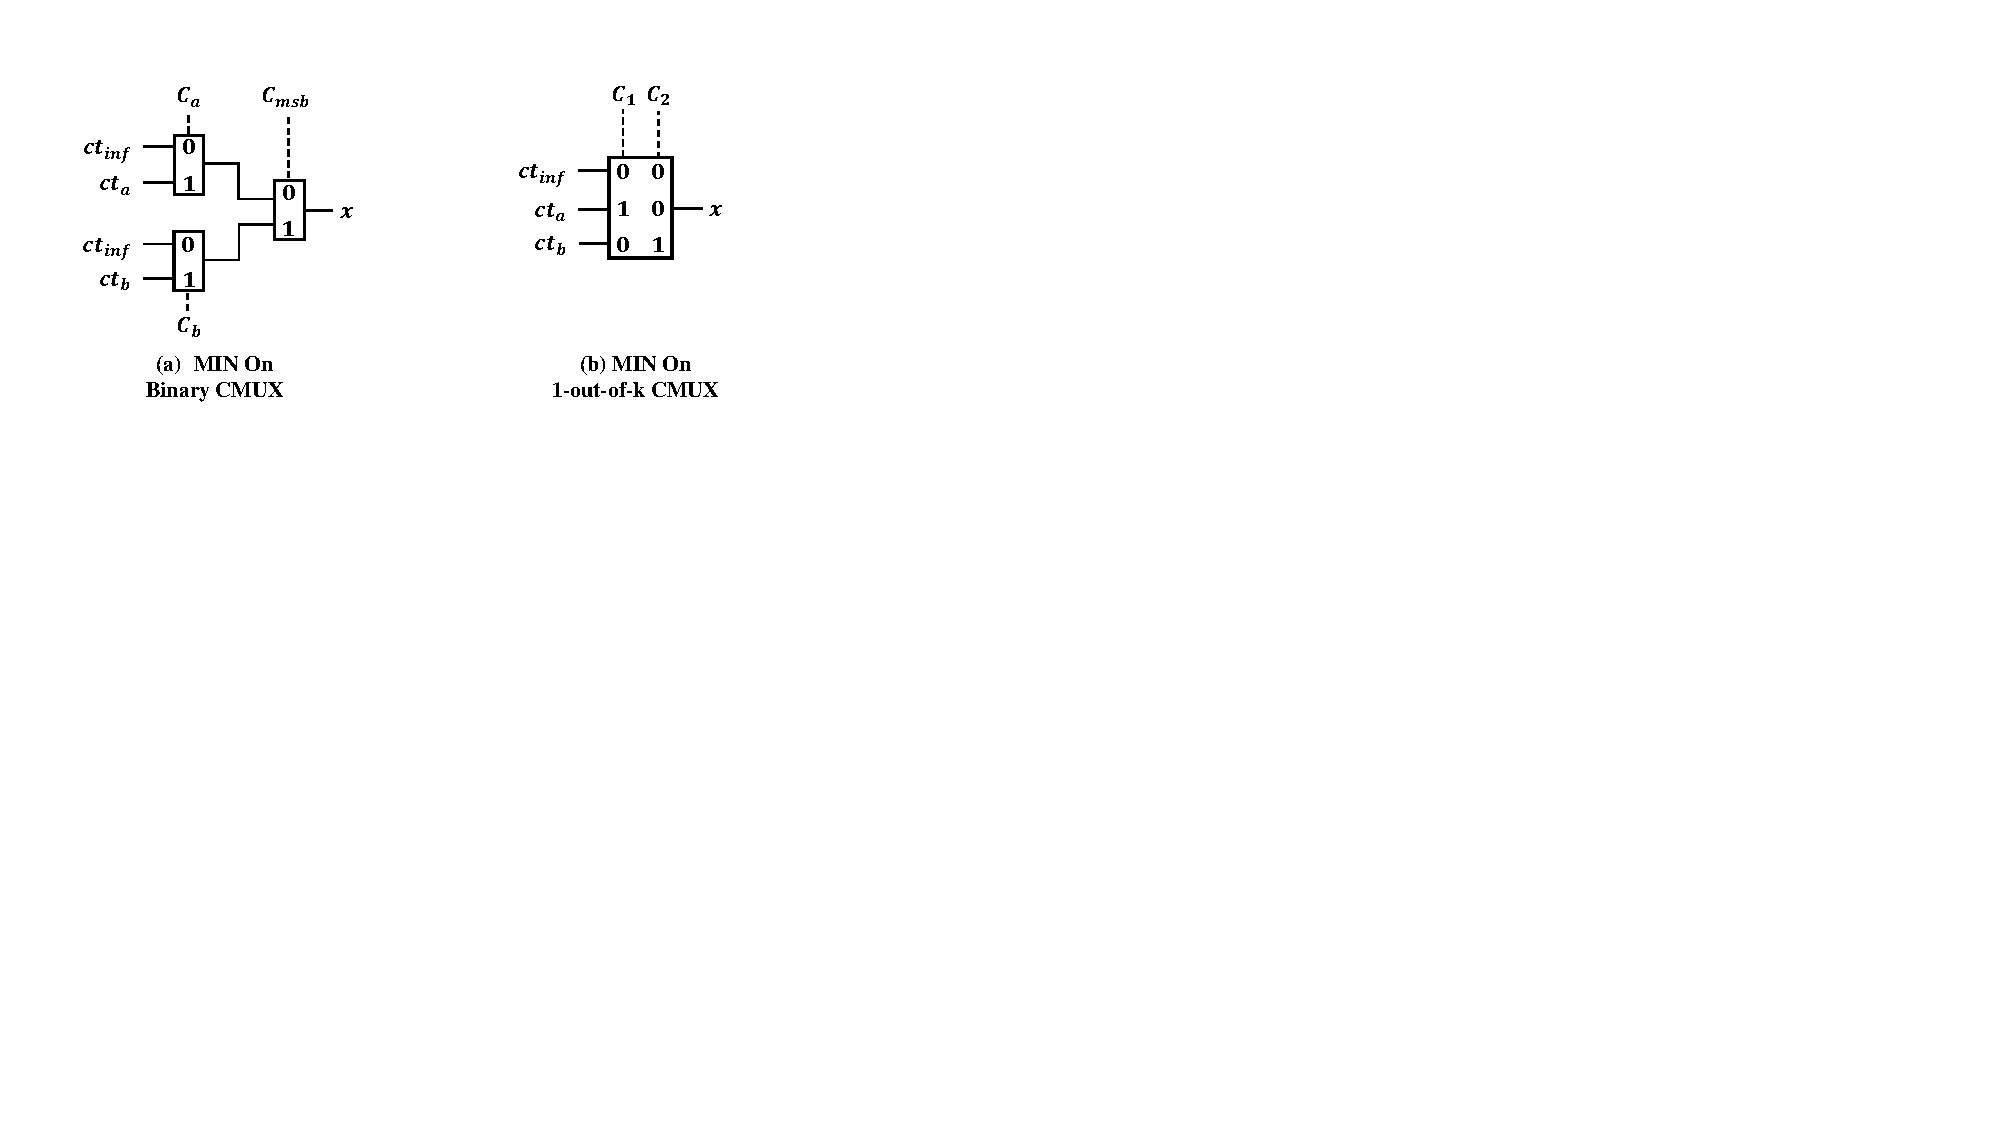
\includegraphics[width=\linewidth]{figure/mincmux.pdf}
   \end{center}
    \vspace{-0.5em}
      \caption{A illustration in query evaluation.} 
   \label{fig: mincmux}
   \vspace{-0.5em}
\end{figure}

\subsubsection{Putting all together}

\subsubsection{Extend to \texttt{ORDER BY}}



\subsection{Complicated SQL Queries}
